A brief introduction into nonlinear continuum mechanics and the relevant governing equations will be presented in this section. 

\subsection{Kinematics: motion and deformation}\label{sec:kinematics}

Let us consider the motion of an EAP with reference configuration $\mathcal{B}_0\in \mathbb{R}^3$ (refer to Figure 1). 
After the motion, the continuum $\mathcal{B}_0$ occupies a deformed configuration $\mathcal{B}\in\mathbb{R}^3$. 
The deformation mapping $\vect{\phi}\left(\vect{X},t\right)$ links a material particle from the reference configuration $\vect{X}\in \mathcal{B}_0$ to the deformed configuration $\vect{x}\in \mathcal{B}$ according to $\vect{x} = \vect{\phi}\left(\vect{X},t\right)$. Associated with $\vect{\phi}$, we define the deformation gradient tensor $\vect{F}\in \text{GL}^{+}(3)$ (or fibre map) \cite{Bonet_book_statics,Gonzalez_book,deSouza_book,Bathe_book} as $\vect{F}=\partial_{\vect{X}}\vect{\phi}$. The later permits to introduce its co-factor  $\vect{H}$ (or area map) and its Jacobian $J$ (or volume map), according to 
%
\begin{equation}\label{eqn:H and J classical}
\vect{H} = \left(\text{det}\vect{F}\right)\vect{F}^{-T};\qquad
J = \text{det}\vect{F},
\end{equation}
%
which can be equivalently re-writen as \cite{deBoer_book,Bonet_cross_product_2016} as
%
\begin{equation}\label{eqn:H and J tensor cross product expression}
	\vect{H}=\frac{1}{2}\vect{F}\Cross\vect{F}; \qquad  J=\frac{1}{3}\vect{H}:\vect{F},
\end{equation}
%
%

\begin{figure}[htbp]
	\begin{center}
		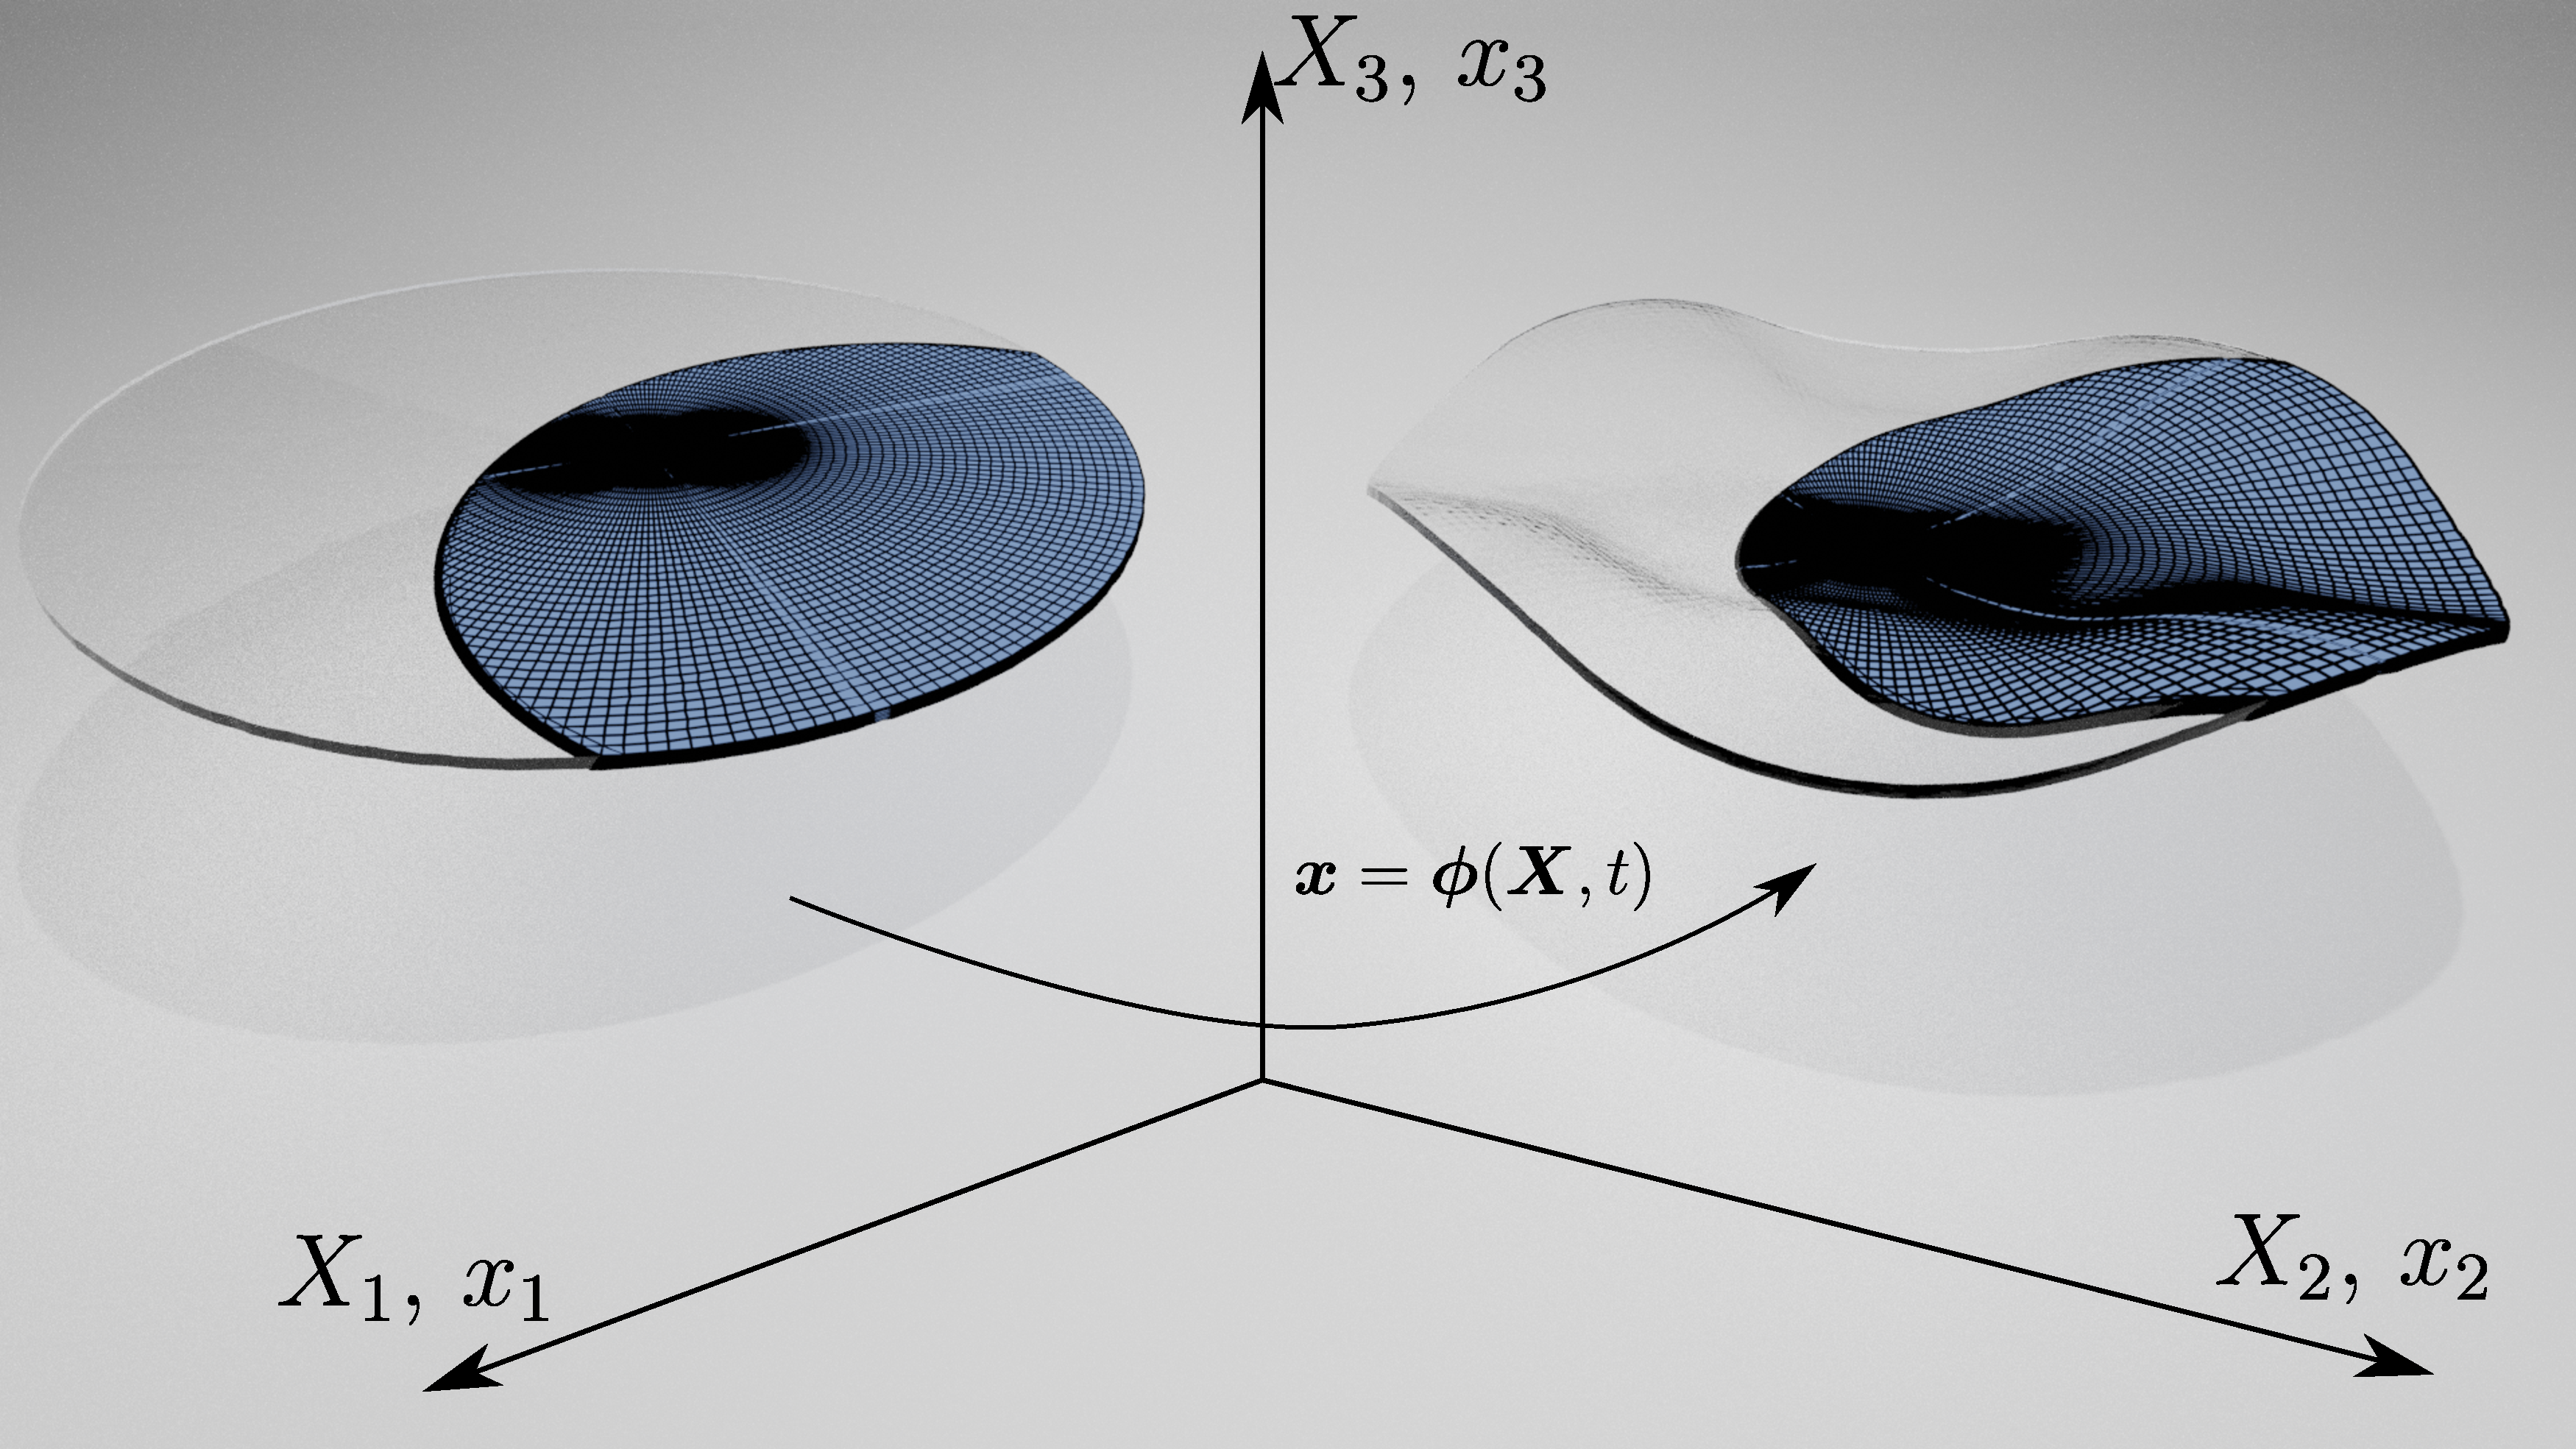
\includegraphics[width=0.6\textwidth]{Figures/InkScape/TheMappingdeLaOstia}
	\end{center}
	\caption{The mapping $\vect{\phi}$ and the reference $\mathcal{B}_0$ (left) and deformed $\mathcal{B}$ (right) configurations.}
	\label{fig:superpotato}
\end{figure}

% \footnote{In addition, throughout the paper, the symbol $(\cdot)$ is used to indicate the scalar product or contraction of a single index $\vect{a}\cdot \vect{b}=a_i b_i$; the symbol $(:)$ is used to indicate double contraction of two indices $\vect{A}:\vect{B}=A_{ij}B_{ij}$; the symbol $(\times)$ is used to indicate the cross product between vectors $[\vect{a} \times \vect{b}]_i=\mathcal{E}_{ijk}a_jb_k$ and the symbol $(\otimes)$ is used to indicate the outer or dyadic product $[\vect{a}\otimes \vect{b}]_{ij}=a_ib_j$.}. 
%As shown in References \cite{Bonet_cross_product_2016,Bonet_polyconvexity_2015}, the definitions of $\vect{H}$ and $J$ in \eqref{eqn:H and J tensor cross product expression}, although equivalent to those in \eqref{eqn:H and J classical}, are very appealing as they yield simpler expressions for their directional derivatives \cite{Bonet_polyconvexity_2015,Bonet_cross_product_2016, Gil_electro_partI_2016,Gil_electro_partII_2016,Gil_electro_partIII_2016, Betsch_EM_thermo_2017}. 

\subsection{Governing equations in nonlinear thermo-mechanics}\label{sec:governing equations}

The behaviour of the EAP is governed by a system of coupled PDEs. These include the conservation of linear momentum  \cite{Gonzalez_book}, which can be recast in a Lagrangian setting as
%
\begin{equation}\label{eqn:local form conservation of linear momentum}
\begin{aligned}
\rho_0\dot{\vect{v}} - \text{DIV}\vect{P} - \vect{f}_0& = \vect{0};&\qquad &\text{in}\,\,\mathcal{B}_0\times [0,T];\\
%
\vect{P}\vect{N}& = \vect{t}_0;&\qquad&\text{on}\,\,\partial_{\boldsymbol{t}}\mathcal{B}_0\times [0,T];\\
%
\vect{\phi} &= \bar{\vect{\phi}};&\qquad & \text{on}\,\,\partial_{\vect{\phi}}\mathcal{B}_0\times [0,T];\\
%
\left.{\vect{\phi}}\right\vert_{t=0}&=\bar{\vect{\phi}}_0;&\qquad
&\text{in}\,\,\mathcal{B}_0;\\
%
\left.\dot{\vect{\phi}}\right\vert_{t=0}&={\bar{\vect{v}}}_0;&\qquad &\text{in}\,\,\mathcal{B}_0,
%#
%
\end{aligned}
\end{equation}
%
where $\rho_0: \mathcal{B}_0\rightarrow \mathbb{R}^{+}$ represents the mass density of the continuum in the reference configuration, $\vect{v}$ the velocity field.
Furthermore, $\vect{f}_0$ represents a body force per unit undeformed volume $\mathcal{B}_0$ and $\vect{t}_0$, the traction force per unit undeformed area applied on $\partial_{\boldsymbol{t}}\mathcal{B}_0\subset \partial \mathcal{B}_0$, such that $\partial_{\boldsymbol{t}}\mathcal{B}_0 \cup \partial_{\vect{\phi}}\mathcal{B}_0 = \partial\mathcal{B}_0$ and $\partial_{\boldsymbol{t}}\mathcal{B}_0 \cap \partial_{\vect{\phi}}\mathcal{B}_0 = \emptyset$. Moreover, $\bar{\vect{\phi}}$ represents the Dirichlet condition for $\vect{\phi}$, $\bar{\vect{\phi}}_0$ and ${\bar{\vect{v}}}_0$ are the initial conditions for the mapping $\vect{\phi}$ and the velocity fields, respectively.
Finally,  local conservation of angular momentum leads to the well-known tensor condition $\vect{F P} = \vect{P}^T\vect{F}^T$, where $\vect{P}$ represents the first Piola-Kirchhoff stress tensor. 
%

The second set of PDEs that govern the behaviour of the EAP comprises the electrostatic form of the Gauss' and Faraday's laws, recast in a Lagrangian setting as follows
%
\begin{equation}\label{eqn:local form Gauss Faraday}
\begin{aligned}
\vect{E}_0& = -\partial_{\vect{X}}\varphi;&\qquad &\text{in}\,\,\mathcal{B}_0\times [0,T];\\
%
\text{DIV}\vect{D}_0 & = -\rho^e_0;&\qquad &\text{in}\,\,\mathcal{B}_0\times [0,T];\\
%
\vect{D}_0\cdot\vect{N}& = -{\omega}^e_0;&\qquad&\text{on}\,\,\partial_{\omega}\mathcal{B}_0\times [0,T];\\
%
{\varphi} &= \bar{{\varphi}};&\qquad & \text{on}\,\,\partial_{{\varphi}}\mathcal{B}_0\times [0,T],
%
\end{aligned}
\end{equation}
%
where $\varphi : \mathcal{B}_0\rightarrow \mathbb{R}$ represents the electric potential, 
 $\rho^e_0: \mathcal{B}_0\rightarrow \mathbb{R}$ is the electric charge per unit volume in the reference configuration 
 and $\omega_0$, the electric charge per unit undeformed area applied on $\partial_{\omega}\mathcal{B}_0\subset \partial \mathcal{B}_0$, such that $\partial_{\omega}\mathcal{B}_0 \cup \partial_{{\varphi}}\mathcal{B}_0 = \partial\mathcal{B}_0$ and $\partial_{\omega}\mathcal{B}_0 \cap \partial_{{\varphi}}\mathcal{B}_0 = \emptyset$. Finally, $\bar{{\varphi}}$ represents the Dirichlet condition for ${\varphi}$. In above equation \eqref{eqn:local form Gauss Faraday}, $\vect{E}_0$ and $\vect{D}_0$ represent the material electric field and electric displacement field, respectively.

Finally, the last coupled PDE governing the behaviour of the EAP is the balance of energy, which in the absence of internal state variables (i.e. plastic strain or viscoelasticity), can be written in a Lagrangian setting as
%
\begin{equation}\label{eqn:local form energy}
\begin{aligned}
\theta\dot{\eta} + \text{DIV}\vect{Q} - R_{\theta} & = 0;&\qquad& \text{in}\,\,\mathcal{B}_0\times [0,T];\\
%
\vect{Q}\cdot\vect{N}& = -Q_{\theta};&\qquad&\text{on}\,\, \partial_{Q}\mathcal{B}_0\times [0,T];\\
%
\theta & = \bar{\theta};&\qquad&\text{on}\,\,\partial_{\theta}\mathcal{B}_0\times [0,T];\\
%%#
\left.{\theta}\right\vert_{t=0}&={\bar{\theta}}_0;&\qquad& \text{in}\,\,\mathcal{B}_0,
\end{aligned}
\end{equation}
%
where $\theta$ is the absolute temperature field and $\eta$ and $\vect{Q}$, the entropy and heat flux per unit undeformed volume $\mathcal{B}_0$, respectively. In addition, $R_{\theta}$  represents the heat source per unit undeformed volume $\mathcal{B}_0$ and $Q_{\theta}$, the heat source per unit undeformed area applied on $\partial_{Q}\mathcal{B}_0\subset\partial\mathcal{B}_0$. In \eqref{eqn:local form energy}, $\partial_{\theta}\mathcal{B}_0$ represents the part of the boundary $\partial\mathcal{B}_0$ where essential temperature boundary conditions are applied such that $\partial_{Q}\mathcal{B}_0\cup\partial_{\theta}\mathcal{B}_0 = \partial\mathcal{B}_0$ and $\partial_{Q}\mathcal{B}_0\cap\partial_{\theta}\mathcal{B}_0 = \emptyset$. 
%
